\section{The Design of Helios}
\label{sec:design}

\subsection{Overview}
Helios is a path-driven execution engine designed to accelerate EVM transaction processing. Its architecture comprises four coordinated components. The Helios Engine orchestrates execution. The Path Cache indexes optimized graphs for reuse. The Path Tracer captures execution traces. The SSA Optimizer compiles them into an optimized intermediate representation. Figure~\ref{fig:helios-architecture} illustrates the system architecture and data flow.

\begin{figure}[!htbp]
    \centering
    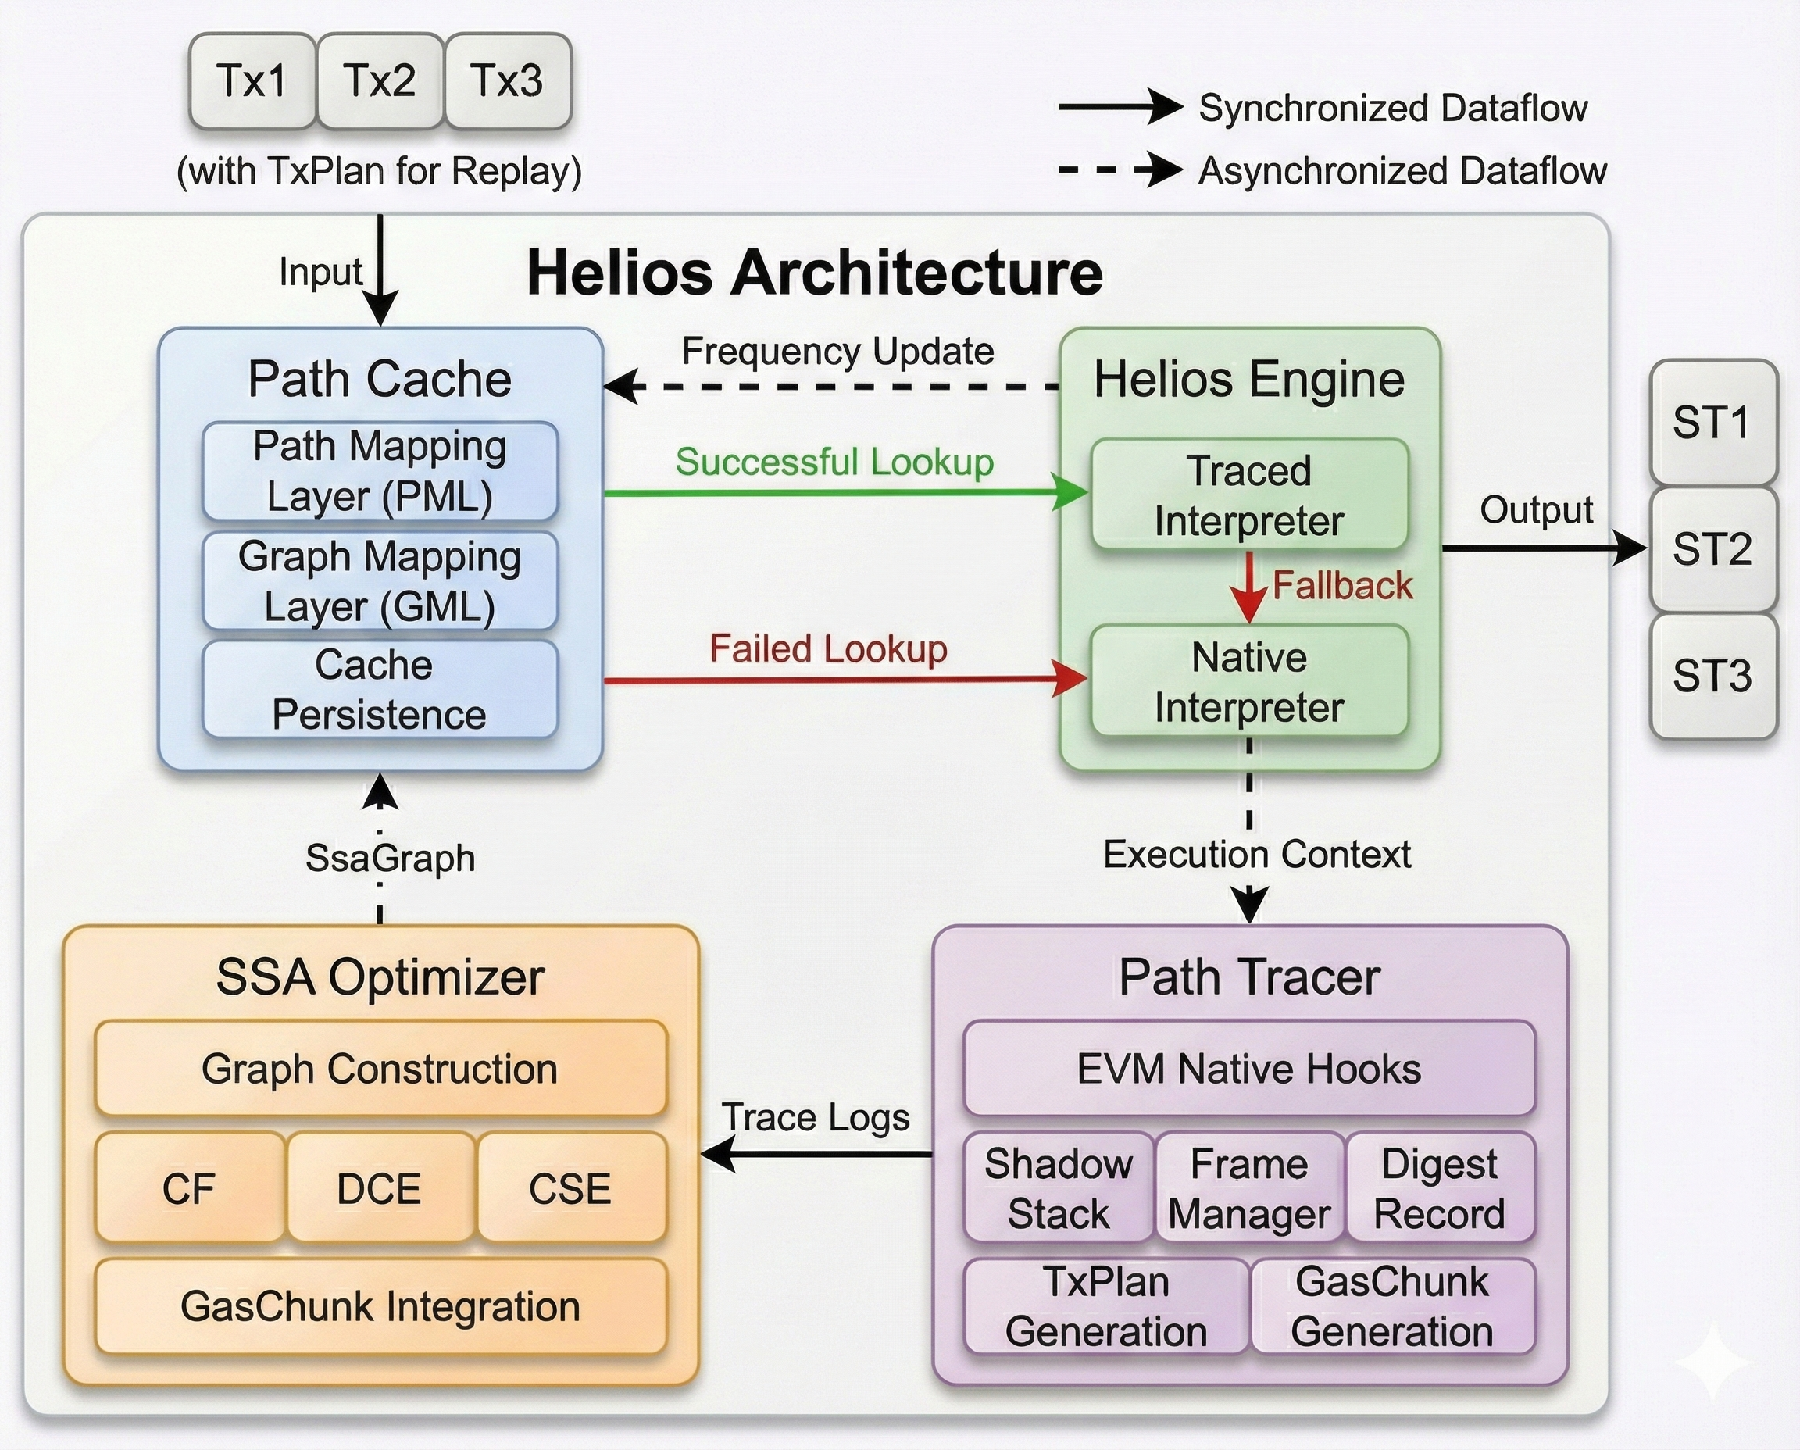
\includegraphics[width=\linewidth]{raw-figures/helios-architecture.pdf}
    \caption{Overview of the Helios architecture.}
    \label{fig:helios-architecture}
\end{figure}

Upon contract invocation, the Helios Engine queries the Path Cache using a path identifier derived from the contract identity and call signature. On a cache miss, the engine delegates execution to the Native Interpreter. This delegation simultaneously initiates an asynchronous optimization pipeline. The Path Tracer captures the raw execution trace as a PathLog, a linear sequence of executed opcodes with their data dependencies. The SSA Optimizer transforms this PathLog into an optimized SsaGraph, a directed acyclic graph that makes data flow explicit. The Path Cache then stores the SsaGraph for future reuse. Running in parallel with the Native Interpreter, this pipeline ensures that optimization never blocks the critical execution path.

On a cache hit, the engine retrieves the corresponding SsaGraph and dispatches it to the Traced Interpreter, which performs speculative execution validated by runtime control-flow guards. An execution failure triggers a fallback to the Native Interpreter and re-initiates the optimization pipeline. Successful execution concludes the transaction with reduced overhead.

Helios supports two operational modes. Online mode targets full nodes and validators handling transactions with unknown paths, where cache misses and guard failures may occur. Replay mode targets archive nodes reprocessing historical blocks. A pre-computed TxPlan guarantees cache hits for every call frame, allowing the engine to bypass control-flow guards and the optimization pipeline for maximum throughput.


\subsection{Key Data Structures}
Helios represents and indexes transaction paths through a small set of data abstractions that govern both Online and Replay modes.

\textbf{Path Representation.}
Execution paths are first captured as a \textit{PathLog}, a raw linear trace produced by the Path Tracer. A PathLog is a sequence of entries, each recording an opcode together with its stack data dependencies, expressed as references to the outputs of preceding operations. The optimization pipeline consumes this representation and transforms it into an \textit{SsaGraph}, a directed acyclic graph whose nodes denote operations and whose edges denote data dependencies. By making data flow explicit and eliminating the implicit EVM stack, the SsaGraph serves as the executable format for the Traced Interpreter.

\textbf{Path Indexing and Retrieval.}
Helios employs a multi-key scheme to locate and reuse SsaGraphs. A \textit{PathDigest} is a 64-bit hash of a path’s opcode sequence acting as a deterministic identifier for the execution logic. A \textit{DataKey} concatenates a contract’s code hash with the PathDigest to uniquely identify the constant table for a specific contract instance. This separation allows multiple contracts with identical bytecode, such as distinct ERC20~\cite{erc20} tokens, to share a single SsaGraph while maintaining separate constant tables. Finally, a \textit{CallSig} is a coarse-grained identifier used for predictive lookup in Online mode, defined as the concatenation of a contract’s code hash and the 4-byte function selector from calldata. A single CallSig may map to multiple PathDigests, corresponding to distinct control-flow branches of the same function, including both successful and revert paths.

\textbf{Execution Metadata.}
Helios maintains additional metadata to coordinate cross-frame execution and reduce runtime overhead. A \textit{Transaction Plan (TxPlan)} is an ordered sequence of PathDigests that records the path taken by each call frame within a transaction. TxPlans are produced during Online execution and indexed by block number and transaction index; in Replay mode, they provide a deterministic guide for fetching the correct SsaGraph for every frame. A \textit{GasChunk} is a precomputed scalar capturing the cumulative static gas cost of the instructions lying between two consecutive gas-accounting opcodes. Attached to the corresponding SsaGraph, GasChunks allow the Traced Interpreter to replace per-instruction gas accounting with a single bulk deduction, thereby reducing overhead while preserving gas-semantic equivalence.

\subsection{Component Design and Implementation}
This section details the internal design and mechanisms of each of Helios's four primary components. It describes how each component fulfills its role in the end-to-end transaction lifecycle, transforming its inputs into the data structures required by the next stage of the pipeline.


\begin{algorithm}[!htbp]
\small
\caption{Shadow Stack Tracing}
\label{alg:shadow-stack-tracing}
\KwIn{$op$: Current EVM opcode}
\KwIn{$S_{evm}$: EVM value stack (after opcode execution)}
\KwIn{$S_{\ell}$: Shadow stack of LSNs tracking value provenance}
\KwOut{$e$: Trace log entry containing the opcode, current LSN, input dependencies, and output value}
\KwOut{Updated $S_{\ell}$}

\tcp{Extract input dependencies from shadow stack}
$D_{in} \gets []$ \\
$k \gets$ \textsc{GetInputCount}$(op)$ \\
\For{$i \gets 1$ \KwTo $k$}{
    $\ell \gets S_{\ell}$.\textsc{Pop}() \\
    $D_{in}$.\textsc{Append}$(\ell)$ \\
}

\tcp{Record output value and assign new LSN}
\eIf{$op$ produces stack output}{
    $v_{out} \gets S_{evm}$.\textsc{Top}() \\
    $\ell_{curr} \gets$ \textsc{NextLSN}() \\
    $S_{\ell}$.\textsc{Push}$(\ell_{curr})$ \\
}{
    $v_{out} \gets \bot$ \tcp*{No output, e.g., POP, JUMP}
    $\ell_{curr} \gets$ \textsc{NextLSN}() \\
}

\tcp{Handle stack manipulation instructions}
\If{$op \in \{\text{\texttt{DUP1}}, \text{\texttt{DUP2}}, \ldots, \text{\texttt{DUP16}}\}$}{
    $d \gets op - \text{\texttt{DUP1}} + 1$ \\
    $\ell_t \gets S_{\ell}[d]$ \tcp*{Peek without pop}
    $S_{\ell}$.\textsc{Push}$(\ell_t)$ \tcp*{Duplicate LSN}
}
\If{$op \in \{\text{\texttt{SWAP1}}, \text{\texttt{SWAP2}}, \ldots, \text{\texttt{SWAP16}}\}$}{
    $d \gets op - \text{\texttt{SWAP1}} + 1$ \\
    $S_{\ell}$.\textsc{Swap}$(0, d)$ \tcp*{Swap LSNs}
}

\tcp{Create log entry}
$e \gets \langle op, \ell_{curr}, D_{in}, v_{out} \rangle$ \\

\Return{$e$}

\end{algorithm}

\subsubsection{Path Tracer}
A lightweight instrumentation component observes native EVM execution to produce the raw PathLog data structure, TxPlan, and GasChunk.

\textbf{Instrumentation mechanism.} The tracer attaches to the EVM hook interface and subscribes to six events, including \texttt{step} and \texttt{step\_end} for opcode execution, \texttt{call} and \texttt{call\_end} for external calls, and \texttt{create} and \texttt{create\_end} for contract creation. This hook-based design decouples the tracer from the interpreter and enables passive observation without changing execution semantics.

To capture stack data dependencies, the tracer maintains a shadow stack mirroring the EVM operand stack but storing 32-bit Log Sequence Numbers or LSNs instead of 256-bit values. Each LSN identifies the operation producing the corresponding value. As detailed in Algorithm~\ref{alg:shadow-stack-tracing}, the tracer pops the required input LSNs to form the dependency list $D_{in}$ on each \texttt{step\_end}, allocates a new LSN for the current opcode, and pushes it if the opcode produces a stack result. For stack-manipulation opcodes such as \texttt{DUP} and \texttt{SWAP} that only reorder values, the tracer applies the same permutation to the shadow stack without creating a new LSN. As a result, only opcodes that actually produce new values become nodes in the PathLog, effectively collapsing substantial stack traffic and yielding PathLog entries that record each operation alongside the LSNs of its true data dependencies.

\textbf{PathDigest Calculation.} PathDigest is a rolling hash updated with each executed opcode using the lightweight FNV-1A algorithm~\cite{fnv1, fnv2}. FNV-1A was chosen for its efficiency, involving simple multiplication and XOR operations. This ensures a unique identifier for each execution path and allows fast incremental updates, enabling efficient path comparison and lookup in the PathCache.

\textbf{Metadata generation.} The tracer also constructs GasChunk and TxPlan metadata. For GasChunks, it treats \texttt{GAS} and terminating opcodes such as \texttt{RETURN}, \texttt{STOP}, \texttt{REVERT}, \texttt{CREATE}, and \texttt{CREATE2} as gas delimiters. It accumulates the static gas cost of instructions between two delimiters and emits a GasChunk with the aggregate cost upon reaching a delimiter. If a path ends without an explicit delimiter, the system inserts a synthetic \texttt{STOP} to close the final chunk.

The TxPlan is built using placeholders. When a new frame is entered via the \texttt{call} or \texttt{create} hook, the tracer appends a placeholder entry. When the frame completes at \texttt{call\_end} or \texttt{create\_end}, it computes the frame's PathDigest and replaces the placeholder. The resulting TxPlan records the final per-frame path sequence in transaction order.

\textbf{Path Validation and Filtering.} To restrict resource allocation to reusable paths, the tracer executes a health check during the \texttt{call\_end} hook by inspecting the frame's exit status. The system discards paths resulting from VM-level exceptions, particularly out-of-gas errors, while retaining deterministic application-level terminations such as successful returns and \texttt{REVERT} operations. This distinction is critical because \texttt{REVERT} paths correspond to reproducible control-flow branches, including failed assertions or balance validations, which exhibit high reusability across transactions. Conversely, VM-level exceptions are non-deterministic and may manifest at any instruction depending on the gas limit. Tracking every potential out-of-gas point for a sequence of $n$ opcodes would generate $O(n)$ distinct failure paths, leading to cache fragmentation without benefiting deterministic execution. Consequently, the tracer formats only deterministically terminated paths into PathLog entries for the SSA Optimizer.

\subsubsection{SSA Optimizer}
A pure-function component transforms a raw PathLog into an optimized, gas-annotated SsaGraph through a pipeline of graph construction, redundancy elimination, gas integration, and final compaction.

\textbf{Graph construction.} For each PathLog entry, the optimizer creates a node in the SsaGraph and connects it to its data-dependency predecessors using the $D_{in}$ LSN list, yielding a graph representation of the linear trace.

\textbf{Optimization passes.} The graph then undergoes three side-effect-aware passes: constant folding, dead-code elimination, and common-subexpression elimination. First, PUSH nodes are converted into constant-table entries and their values are propagated through side-effect-free nodes; computations that become fully constant are removed and recorded as constants. Second, a backward scan from side-effecting nodes removes any node whose result is unused, iterating to a fixed point. Third, the optimizer merges redundant side-effect-free operations by assigning each one a fingerprint consisting of its opcode and input LSNs; nodes with identical fingerprints are unified and all consumers are redirected to the canonical node.

\textbf{GasChunk Integration.} Following the optimization pipeline, the optimizer integrates the GasChunk metadata collected by the Path Tracer. It retrieves the list of GasChunks from the PathLog and attaches each pre-computed gas cost to its corresponding delimiter node within the SsaGraph. This annotation embeds the gas accounting information directly into the executable graph structure.

\textbf{Graph Compaction and Output.} In the final stage, the optimizer physically deletes all nodes previously marked as REMOVED to produce a compact graph. It finalizes the constant table, containing all immediate values and folded constants from the optimization phase. The resulting SsaGraph, its constant table, and associated identifiers are then transmitted to the Path Cache for storage.

\subsubsection{Path Cache}
A two-tier architecture separates prediction logic from canonical storage to efficiently support both probabilistic Online lookups and deterministic Replay retrieval.

\textbf{Tiered Architecture.} The Path Mapping Layer (PML) operates as a frequency-based prediction index for Online mode. It maintains a dual-index structure for each CallSig comprising a frequency map $M_{freq}$ for $O(1)$ access and a priority queue $I_{sorted}$ for $O(\log k)$ maximum frequency retrieval. To minimize guard validation overhead, the PML prioritizes precision by returning a prediction only if a single \textit{PathDigest} holds the unique maximum frequency. The Graph Mapping Layer (GML) acts as the deterministic backing store mapping PathDigests to reusable SsaGraphs and DataKeys to contract-specific constant tables.

\begin{algorithm}[t]
\small
\caption{Online Mode: Path Lookup}
\label{alg:online-lookup}

\textbf{Notation:} $\mathcal{S}_{\sigma}$ denotes a PathStore for CallSig $\sigma$, maintaining $M_{freq}$ (PathDigest $\to$ frequency map) and $I_{sorted}$ (frequency $\to$ PathDigest set, sorted index).

\KwIn{$\sigma$: CallSig (code hash $\|$ function selector)}
\KwIn{$h_c$: Contract code hash for DataKey construction}
\KwIn{$\mathcal{P}$: Path Cache with PML and GML layers}
\KwOut{$(G, C, \ell)$: Cached graph, constant table, and PathDigest; or $\bot$ if prediction fails}

\tcp{Phase 1: Query Path Mapping Layer for hot path}
\If{$\sigma \notin \mathcal{P}.PML$}{
    \Return{$\bot$} \tcp*{Cold start: CallSig never observed}
}

$\mathcal{S}_{\sigma} \gets \mathcal{P}.PML[\sigma]$ \tcp*{Retrieve PathStore}
\textsc{AcquireReadLock}($\mathcal{S}_{\sigma}$) \\

\tcp{Get unambiguous maximum frequency path}
$(f_{max}, P_{max}) \gets I_{sorted}.\textsc{LastEntry}()$

\If{$|P_{max}| \neq 1$}{
    \textsc{ReleaseReadLock}($\mathcal{S}_{\sigma}$) \\
    \Return{$\bot$} \tcp*{Ambiguous: multiple paths share max frequency}
}

$\ell \gets P_{max}.\textsc{First}()$ \tcp*{Extract the unique hot path}
\textsc{ReleaseReadLock}($\mathcal{S}_{\sigma}$) \\

\tcp{Phase 2: Query Graph Mapping Layer for artifacts}
\If{$\ell \notin \mathcal{P}.GML.graphs$}{
    \Return{$\bot$} \tcp*{Path not yet optimized}
}

$k_{data} \gets h_c \| \ell$ \tcp*{Construct DataKey}

\If{$k_{data} \notin \mathcal{P}.GML.data$}{
    \Return{$\bot$} \tcp*{Constant table missing}
}

$G \gets \mathcal{P}.GML.graphs[\ell]$ \\
$C \gets \mathcal{P}.GML.data[k_{data}]$ \\

\Return{$(G, C, \ell)$} \tcp*{Successful prediction}

\end{algorithm}


\textbf{Query and Update Protocols.} Query logic adapts to the operational mode. In Online mode, as detailed in Algorithm~\ref{alg:online-lookup}, the engine requests a high-confidence prediction from the PML. A successful hit yields a PathDigest that combines with the contract code hash to retrieve execution artifacts from the GML. In contrast, Replay mode bypasses the PML to perform direct lookups in the GML using the TxPlan.

\begin{algorithm}[!htbp]
\small
\caption{Path Frequency Update (Feedback Loop)}
\label{alg:path-frequency-update}

\textbf{Notation:} Symbols follow Algorithm~\ref{alg:online-lookup}. Additionally, $k$ denotes the number of distinct frequencies in $I_{sorted}$.

\KwIn{$\sigma$: CallSig corresponding to the executed path}
\KwIn{$\ell$: PathDigest that was successfully executed}
\KwIn{$\mathcal{P}$: Path Cache with PML}
\KwOut{Updated frequency statistics in $\mathcal{S}_{\sigma}$}

\tcp{Retrieve or create PathStore for this CallSig}
$\mathcal{S}_{\sigma} \gets \mathcal{P}.PML.\textsc{GetOrCreate}(\sigma)$ \\
\textsc{AcquireWriteLock}($\mathcal{S}_{\sigma}$) \tcp*{Exclusive access for update}

\tcp{Phase 1: Get current frequency}
$f_{old} \gets M_{freq}.\textsc{Get}(\ell)$ \textbf{or} $0$ \tcp*{Default to 0 for new paths}
$f_{new} \gets f_{old} + 1$ \tcp*{Increment with saturation}

\tcp{Phase 2: Update sorted index}
\If{$f_{old} > 0$}{
    $P_{old} \gets I_{sorted}[f_{old}]$ \tcp*{Get old frequency bucket}
    $P_{old}.\textsc{Remove}(\ell)$ \\
    \If{$P_{old} = \emptyset$}{
        $I_{sorted}.\textsc{Remove}(f_{old})$ \tcp*{Clean empty bucket}
    }
}

\tcp{Phase 3: Update sorted index}
$P_{new} \gets I_{sorted}.\textsc{Entry}(f_{new}).\textsc{OrInsertEmpty}()$ \\
$P_{new}.\textsc{Insert}(\ell)$ \\

\tcp{Phase 4: Update frequency map}
$M_{freq}[\ell] \gets f_{new}$ \\

\textsc{ReleaseWriteLock}($\mathcal{S}_{\sigma}$) \\

\end{algorithm}


Cache updates occur through two mechanisms formalized in Algorithm~\ref{alg:path-frequency-update}. First, the SSA Optimizer populates the GML and initializes the PML entry upon generating a new graph. Second, successful online executions trigger a feedback loop where the engine signals the PML to increment the path's access frequency. This mechanism adapts predictions to evolving traffic patterns. Fine-grained read-write locks manage concurrency by permitting parallel reads for hot path prediction while bounding write contention.


\textbf{Persistence and Recovery.} The system serializes cache state to disk via periodic checkpoints to ensure durability. A configurable pruning policy manages storage by evicting CallSigs below a frequency threshold. Upon node restart, indices are reconstructed from checkpoints in $O(N \log k)$ time to enable immediate high-accuracy prediction. The system handles paths absent from the checkpoint via lazy regeneration.

\subsubsection{Helios Engine}
A central orchestrator supports transaction execution in both Online and Replay mode. 

It integrates with the host EVM client by replacing the per-frame execution loop while reusing the client's state and memory management. In our Revm integration, Helios inherits arena-based memory allocation, cached and prewarmed storage access, and the transaction-local journal for atomic commits. This allows the engine to focus on optimizing intra-frame computation while leaving state handling unchanged. For each frame, Helios chooses between its Traced Interpreter and Native Interpreter based on the execution mode and the Path Cache output.

\textbf{Transaction-scoped execution.} Helios executes at transaction granularity. If a traced execution encounters a cache miss, guard violation, or out-of-gas condition, the engine discards all partial work and restarts the transaction on the Native Interpreter. This design avoids fine-grained checkpointing or rollback and relies on the EVM's transaction-level atomicity for correctness.

\input{algorithm/traced-execution}

\textbf{Traced Interpreter.} When the Path Cache returns a valid SsaGraph, the engine dispatches execution to the Traced Interpreter, whose loop is given in Algorithm~\ref{alg:traced-execution}. It differs from a standard EVM interpreter in three ways.

First, it replaces the EVM stack with a register-like array indexed by LSN. Each SsaGraph node writes its result to its assigned slot, and consumers read operands directly from this array, eliminating DUP/SWAP and other stack manipulation overhead.

Second, in Online mode, it enforces speculative control-flow guards. Before executing JUMP or JUMPI, the interpreter computes the runtime target and checks it against the cached target in the SsaGraph. Any mismatch triggers an immediate transaction-level fallback. In Replay mode, all control-flow targets are fixed by the TxPlan, so these guards are never violated by construction.

Third, it uses chunked gas accounting for static-cost instructions. Instructions accumulate static cost within their GasChunk, and the interpreter deducts the aggregated amount at delimiter nodes in a single operation. Instructions with dynamic gas cost perform individual gas calculations and deductions, preserving exact gas semantics while reducing the number of checks on the hot path.

\subsection{Security Considerations}

Beyond the JIT Bomb resistance established through the path-driven paradigm in \S\ref{sec:background_motivation}, Helios's design inherently mitigates path explosion attacks. An adversary might attempt to degrade system performance by constructing malicious contracts that generate millions of unique execution paths for a single function signature, potentially flooding the cache and consuming resources.

Helios's architecture naturally defends against this attack vector through three complementary mechanisms. The frequency-based Path Mapping Layer ensures that only paths with demonstrated reusability are predicted and accelerated. Attack-generated paths remain perpetually classified as cold paths due to low execution counts, excluded from the prediction model. The checkpoint pruning mechanism evicts CallSigs with access frequencies below a configurable threshold, preventing malicious cold paths from consuming long-term storage while retaining legitimate hot paths. The transaction-scoped execution model ensures that cache misses simply trigger fallback to the Native Interpreter, maintaining correctness and baseline performance for unpredicted paths.

Consequently, path explosion attacks impose only bounded costs on asynchronous tracing and temporary cache occupancy without degrading performance for legitimate transactions. This robustness emerges naturally from the frequency-based filtering and bounded resource allocation inherent to Helios's design.

